\section{Многопроцессорные вычисления}

\subsection{Многопроцессорные системы, их использование для решения задач
фильтрации}   
Одним из наиболее интересных направлений развития современной вычислительной
техники являются многопроцессорные системы. В настоящее время происходит фантастически
быстрый рост мощности
вычислительной техники, что дает реальную возможность
приступить к моделированию тех задач, которые ранее были недоступны для
численного решения. Но, с другой стороны, пришлось столкнуться с той ситуацией,
когда высокопроизводительная многопроцессорная вычислительная техника используется 
лишь на небольшую часть своих потенциальных возможностей. Эта проблема в первую очередь 
связана с трудностями адаптации алгоритмов решения к архитектуре многопроцессорных 
ЭВМ с распределенной памятью. 
 
Многопроцессорные системы можно разделить на 2 класса - системы с общей памятью
и системы с распределенной памятью.
\begin{enumerate}
\item  Системы с общей памятью. 

С точки зрения программиста привлекательно выглядят системы с общей памятью.
Разбитая на взаимодействующие процессы (нити) программа в большинстве таких
систем автоматически распределяется по доступным процессорам системы. Достаточно
широкий круг последовательных алгоритмов может быть успешно адаптирован к
функционированию на системах с общей, или, что тоже самое, разделяемой памятью.

Однако у систем с общей памятью есть ряд существенных недостатков:
\begin{itemize}
\item относительно небольшое число процессоров;
\item отсутствие возможности наращивания числа процессоров - масштабируемости;
\item пиковая производительность систем с общей памятью ниже пиковой
производительности систем с раздельной памятью;
\item высокая, относительно аналогичных по производительности систем с
раздельной памятью, стоимость.
\end{itemize}
Сказанное выше приводит к тому, что сконструированная система, как правило, не
предусматривает возможности существенного наращивания числа процессорных узлов и
обуславливает крайне высокую, относительно рассматриваемых систем с раздельной
памятью, стоимость.
 
\item Системы с распределенной памятью.
 Масштабируемые системы массового параллелизма конструируют на основе
объединения каналами передачи данных процессорных узлов, обладающих своей
локальной оперативной памятью, недоступной другим процессорам. Обмен данными
между процессорами при таком подходе возможен лишь с помощью сообщений,
передаваемых по каналам связи. Такая схема обладает рядом преимуществ по
сравнению с системами, построенными на основе общей памяти. Подчеркнем основные
преимущества систем с распределенной памятью:
\begin{itemize}
\item сравнительно низкая стоимость;
\item масштабируемость - возможность построения систем требуемой
производительности и наращивания их мощности за счет установки дополнительных
процессоров.
\end{itemize}

Системы с раздельной памятью, по-видимому, всегда будут лидировать по показателю
пиковой производительности, поскольку любые новые однопроцессорные (или
многопроцессорные на основе общей памяти) системы могут быть легко объединены
сетью и использованы в качестве многопроцессорных комплексов с раздельной
памятью. 

Но, к сожалению, эффективное использование систем с распределенной памятью
требует значительных усилий со стороны разработчиков прикладного обеспечения и
возможно далеко не для всех типов задач. Для широкого круга хорошо
зарекомендовавших себя последовательных алгоритмов не удается построить
эффективные параллельные аналоги.
\end{enumerate}


\subsection{Параллелизм}

В рассматриваемой работе параллельный алгоритм строится по принципу
геометрического параллелизма.
Геометрический параллелизм является одним из наиболее распространенных типов
параллелизма, применяемых при решении задач, где имеется большое число
однородных действий над однородными данными, которые можно так разбить на
группы, что при обработке каждой группы не потребуется обращений к данным из
других групп, за исключением их малого числа.

Последнее свойство будем называть свойством локальности алгоритма. Локальный
алгоритм допускает разбиение данных на части по числу процессоров, при котором
обработку каждой части осуществляет соответствующий процессор. Этот подход
весьма эффективен при условии, что действия, выполняемые одним процессором,
зависят лишь от небольшого, ограниченного объема данных, расположенных на других
процессорах. Желательно, чтобы эти "'чужие"' данные были локализованы на
ограниченном, небольшом количестве процессоров.

В данной работе рассматривается подход, согласно которому к традиционному
языку программирования(C/C++) добавляются специальные
библиотеки функций.

Основная причина использования дополнительных, специально разработанных
библиотек - обеспечение переносимости создаваемых прикладных продуктов.

В настоящее время широкое распространение получил стандарт разработки
параллельных программ MPI (Message Passing Interface - интерфейс передачи
сообщений) для систем с разделенной памятью. 
В данной работе он используется для осуществления передачи
сообщений между процессорами.

\subsection{О технологии CUDA}
В настоящее время графические процессоры (GPU -- Graphics Processing Unit)
являются оптимальной по соотношению цена-производительность параллельной 
архитектурой с общей памятью. Причина высокой производительности видеокарт 
в том, что они изначально были сконструированы для одновременного применения
одной и той же шейдерной функции к большому числу пикселей, или, другими 
словами, для высокопроизводительных параллельных вычислений.

До недавнего времени использовать вычислительный мощности видеокарт было
крайне неудобно, так как программисту необходимо было
овладеть шейдерным языком программирования, соответствующему коду,
выполняемому на GPU. Причем, в графических API полностью отсутствует
возможность взаимодействия между параллельно обрабатываемыми пикселами,
что в графике действительно не нужно, а для вычислительных задач оказывается довольно
желательным. Ситуация изменилась, когда появились средства разработки
GPGPU-приложений(General-Purpose computing on Graphics Processing Units). 
В качестве таких средств выступают CUDA, OpenCL, Dx11 Compute
Shaders. 

Предложенная компанией Nvidia технология CUDA (Compute Unified Device Architecture) -- 
заметно облегчает написание GPGPU-приложений. Данная технология предназначена для
разработки приложений для массивно-параллельных вычислений. Все программы пишутся на
"'расширенном"' языке C, есть хорошая документация, инструменты, набор библиотек,
поддерживается кроссплатформенность. CUDA является полностью бесплатной и уже 
приобрела широкую популярность в научных кругах.

CUDA строится на концепции, что GPU выступает в роли массивно-параллельного
сопроцессора к CPU. При этом последовательный код выполняется на CPU,
а для массивно-параллельных вычислений соответствующий код выполняется на
GPU как набор одновременно выполняющихся нитей(потоков, threads).

Таким образом, GPU рассматривается как специализированное вычислительное устройство,
которое:
\begin{enumerate}
  \item является сопроцессором к CPU;
  \item обладает собственной памятью;
  \item обладает возможностью параллельного выполнения огромного количества отдельных
  нитей.
\end{enumerate}

В данной работе рассматривается применение технологии CUDA к задачам 
трехфазной фильтрации.

\subsection{Результаты расчетов в многопроцессорном случае}

Для вычислений в многопроцессорном случае и оценки их эффективности
рассматривались такие же задачи, как и для однопроцессорного. Константы моделей
совпадают.

Программа, реализующая параллельный вариант вычислений, написана на языке
программирования С/C++ (в среде Visual Studio 2010) с помощью средств
параллельного программирования MPI (а именно MPICH2) и CUDA. Она является
кроссплатформенной и запускается как в системах Windows, так и Linux, что
позволяет использовать её на различных кластерах. Также она является составной
частью модульного комплекса программ для решения задач фильтрации. 

Для распараллеливания задачи использован геометрический параллелизм: исходная 
область(ортогональная) разбивается на число подобластей (параллелепипедов или квадратов), 
кратное числу
используемых процессоров, причем разбиение области производится по горизонтали.
При таком подходе решение задачи в каждой подобласти осуществляет
соответствующий процессор, и все процессоры равномерно нагружены. Обмен данными
между процессорами осуществляется  на границах подобластей.

При использовании графических ускорителей деление области также осуществляется
методом геометрического параллелелизма в соответствии с геометрией GPU. 
	
При расчете явной схемы процессоры обмениваются сразу всеми пограничными
точками, что дает экономию времени при передаче. 

В процессе работы над дипломом на кластере К-100, ИПМ им. М.В.Келдыша РАН
было протестировано несколько тестовых задач. Ускорения и эффективность вычислений
были подробно проанализированы на примере тестовой задачи 1, описанной в соответствующем
разделе. 

\subsubsection{Результаты применения библиотеки MPI}

На приведенных графиках (рис.~\ref{graph1}-\ref{graph2}) изображены
ускорения и эффективности вычислений в зависимости от числа расчетных узов сетки для 
различного числа процессоров.

\begin{figure}[!h]\center
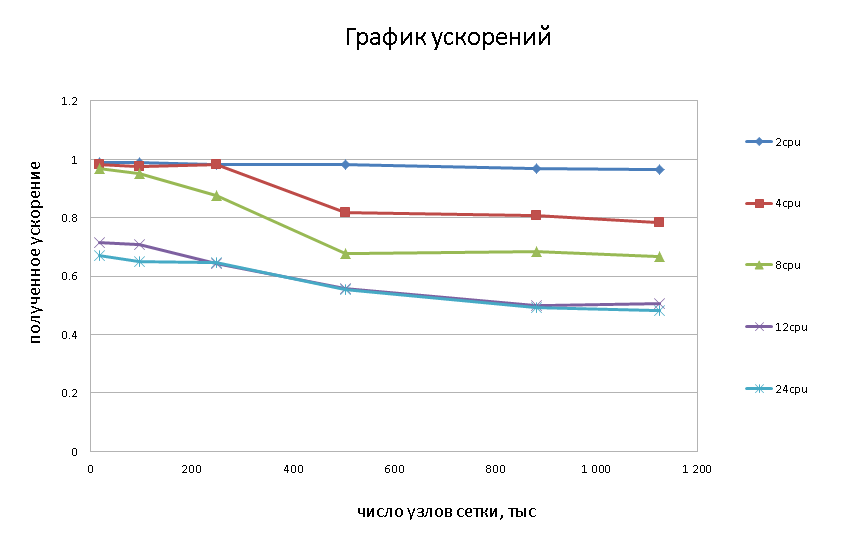
\includegraphics[width=15cm]{scpu.png} 
\caption{Ускорение вычислений в зависимости от числа расчетных узов сетки для разного количества процессоров}\label{graph1}
\end{figure}
\begin{figure}[!h]\center
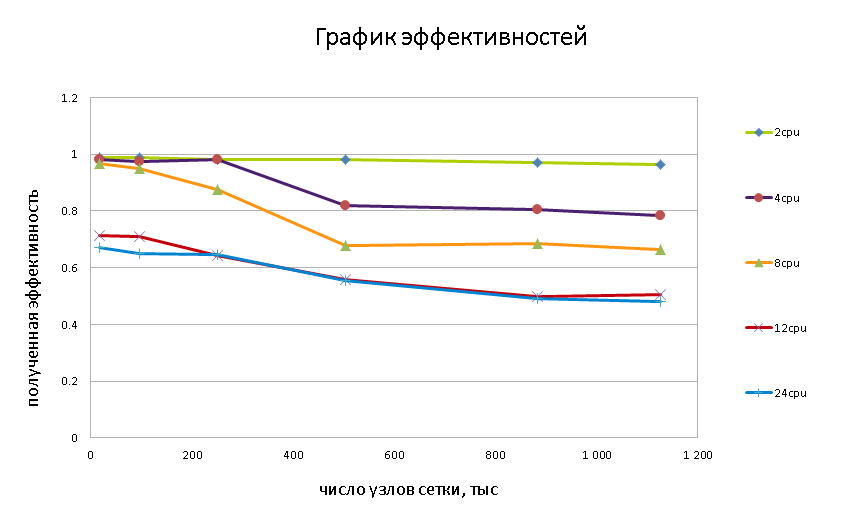
\includegraphics[width=15cm]{Effcpu.png} 
\caption{Эффективность вычислений в зависимости от числа расчетных узов сетки для разного количества процессоров}\label{graph2}
\end{figure}

Спад эффективности при увеличении числа процессоров обусловлен значительным
ростом числа узлов сетки, подлежащих обмену между вычислителями.
Ситуация может быть улучшена разбиением области по всем направлениям осей
координат, что планируется сделать в дальнейшем.

\subsubsection{Результаты совместного применения библиотек CUDA и MPI}
На одной видеокарте кластера К-100 одновременно удается разместить около 6.2 млн узлов
расчетной сетки. На небольших числах узлов при расчетах на одной видеокарте ускорение составляет 
порядка 30 раз. Наибольшие ускорения удается получить при одновременном использовании
нескольких видеокарт при загрузках памяти близких к полным. Обмен соседними значениями
производится через загрузку-выгрузку данных с GPU на CPU и обмен данными между CPU с помощью MPI.
На приведенном графике (рис.~\ref{graph3}) изображены
ускорения вычислений в зависимости от числа расчетных узов сетки. Каждому значению на 
графике соответствует от 1 до 6 графических плат, соответственно.
\begin{figure}[!h]\center
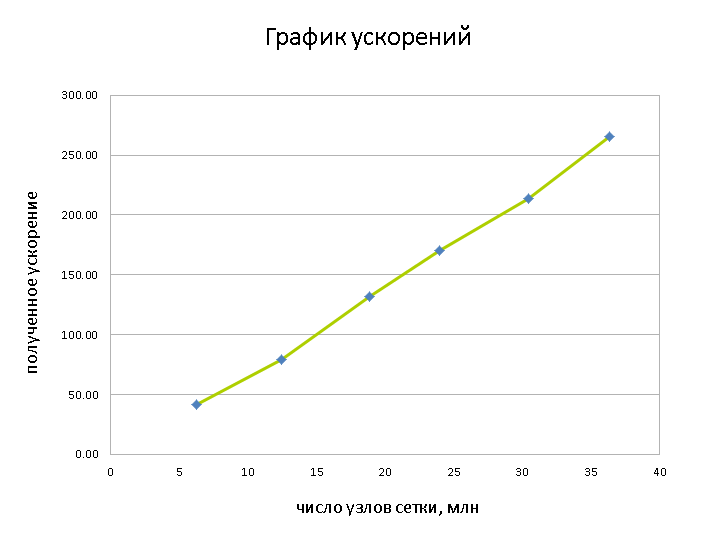
\includegraphics[width=16cm]{sgpu.png} 
\caption{Ускорение вычислений в зависимости от количества точек расчетной области(число графических ускорителей меняется от точки к точке -- от 1 до 6).}\label{graph3}
\end{figure}

Таким образом, в результате использования кластера с гибридной архитектурой были
получены ускорения в 265 раз, при этом на К-100 было задействовано два расчетных узла 
из имеющихся 64 для проведения расчетов на сетке из 36млн точек(на однин узел
приходится 12CPU и 3GPU).
Полученные результаты позволяют предположить, что столь значительные ускорения
расчетов позволят перейти к рассмотрению более широкого круга сложных
вычислительных задач.
